%*******************************************************************************
%*********************************** First Chapter *****************************
%*******************************************************************************

\chapter{Introduction} 


Vehicle makes our life easier by bringing us travel convenience, 
but it also produces problems such as travel cost, carbon pollution, 
car accident and road congestion.
In 2015, about 140.43 billion gallons of gasoline were consumed in the United States. 
Also, according to the US Census Bureau, there are about ten million car accidents every year.
It has been shown that most car accidents are mainly 
caused by dangerous driving behaviors and human mistakes \cite{progressive}. 
These problems are caused by the lack of understanding, monitoring 
and careful control on vehicle dynamics. 
Better understanding and control on vehicle dynamics
can not only reduce car accidents \cite{progressive}, 
but also improve fuel efficiency \cite{morganstanley2013}. 


There has been active efforts to achieve better understanding on
human driving behaviors and better control on vehicles. 
One such example is to use driverless car system to 
replace human drivers \cite{googledriverlesscar, kumar2012carspeak,
urmson2008autonomous,litman2013autonomous}. 
However, it takes time for self-driving systems to be robust enough to 
replace traditional vehicles. 
Also, it is unlikely that self-driving
systems are going to ever achieve perfect accuracy under all
conditions.
Meanwhile, some researchers are using existing technologies to assists human drivers
in user-operated vehicles are more critical for safe 
and efficient driving activities \cite{you2013carsafe, wang2013sensing, chen2015invisible, uber}. 
Also, there are in-vehicle systems that assist human drivers with some driving functionalities, 
e.g., cruise control \cite{bengtsson2001adaptive, cruise_control} and emergence braking system \cite{emergency_brake} etc. 
However, there are many questions that have not been answered: 
what is the accuracy of smartphone sensors to capture driving behaviors?
how to assist human drivers to achieve fuel efficient and safe driving?
how to make self-driving systems more reliable? 


With many open questions in mind, we ask a high-level question in this proposal: 

\emph{how can we build sensing and control system blocks for modern vehicles to
monitor, assist or even replace human drivers in
improving driving performance and experience?}


To answer this question, we explore the sensing and control capabilities
of commodity hardwares and how to utilize them on modern vehicles. 
For example, we can use smartphone to sense and capture 
various driving behaviors, 
based on which we can evaluate driving performance. 
We can also access vehicle parameters from OBD 
port \cite{obd} to evaluate our driving behavior detection algorithms. 
We implemented a smartphone application called DriveSense to collect
data and verify our algorithms. 
We also present a control system called EcoDrive that 
leverages drive-by-wire technology to control fuel injection
rate to find a tradeoff between travel time and fuel efficiency. 
To handle occational self-driving system failures, 
we present a live streaming and remote control framework
called RTDrive to augment self-driving systems. 


\section{DriveSense: Practical Driving Analytics with Smartphone Sensors}



Smartphone-based sensing has opened up a whole gamut of applications and services
for road safety, such as driving behavior and driver distraction monitoring. 
One such application is the ability to independently monitor driving behavior --- how well is one
driving the vehicle, e.g., aggressive driving actions, such as rough acceleration, hard brakes, and lane changes, and more.
The popularity of smartphones and built-in Inertial Measurement Unit (IMU) sensors enable
a low-cost way of monitoring such behaviors and actions.
For example, Cambridge Mobile Telematics \cite{cmt} 
develops a smartphone
app to capture driving behaviors and monitor driver
distractions.
The well-known ride-sharing company Uber announced
it will start tracking Uber drivers' driving behaviors
with their smartphones and give them feedbacks that are more detailed than 
the five-star rating customers leave for each driver \cite{uber}.

The general approach to monitoring such vehicle motion (and drive) parameters is to use an accelerometer in a mobile device
 to measure the three-dimensional acceleration
and using a gyroscope to measure the three-dimensional relative rotation speed.
The accelerometer can be used to sense vehicular speed \cite{hansenspeed}
by eliminating estimation errors at reference points where 
ground truth vehicular speed is known.
The gyroscope can be used to detect turns to determine
driver phone use by comparing centripetal accelerations with 
a reference point \cite{wang2013sensing}, 
and it can also be used to track drivers' 
other steering activities \cite{chen2015invisible}.
Calculating the exact orientation of the phone is an important step in enabling estimation of such motion parameters.
Prior work has dealt with different variants of this problem ---  the absolute coordinates estimation problem (orientation relative
to flat earth surface)  \cite{zhou2014use}
and the relative coordinates estimation problem (orientation relative to the orientation of the vehicle which depends on 
the grade and slope of the road) \cite{wang2013sensing, chen2015invisible}.
Both are challenging tasks due to the low accuracy 
and accumulated errors of IMU sensors \cite{zhou2014use}.
Most in-vehicle applications use the relative coordinates estimation 
and depend on coordinate alignment,
which essentially aligns the coordinates of the smartphone to the car \cite{wang2013sensing, chen2015invisible, hansenspeed}. 
In our evaluation, we found that such prior work is not able to accurately estimate
road slope gradients which leads to increased errors in estimating vehicle motion
parameters. Further, the coordinate alignment process usually needs time to
converge and a fast convergence time is desirable in many real-time settings.

\iffalse
But none of those work addressed the problems caused by road slope
and the method to estimate slope gradients before and after coordinate
alignments.
Also, it is still an open question that how fast 
alignment algorithm can converge, e.g., if an algorithm requires the whole
trip to train the algorithm, then it can not be used in real-time applications for short trips.
\fi


In this section, we study the impact of road slopes on estimating various vehicle motion
parameters, especially the acceleration related ones. This is the central problem for
vehicle motion sensing using such mobile devices because many roads are never perfectly
level and even gentle slope of roads can lead to significant inaccuracies.
Investigating this further, we find that there
are three related issues.
First, we use a real-world driving trace to show that
even a perfectly aligned smartphone may overestimate or
underestimate brakes and accelerations due to the gravitational
effect.
When a car is parked on a slope, the linear acceleration
of the heading direction should be zero, 
but the accelerometer will 
sense the gravity component  in the same direction and conclude
the car is accelerating or decelerating on upslope or downslope. 
Therefore, the heading direction component of the accelerometer may be overestimated or underestimated.
Second, we also show that the gravitational effect can prolong the training time
of coordinate alignment and lower alignment accuracy. 
So, it is necessary to estimate the slope gradients even before
coordinate alignment is fully conducted.
Third, estimating slope gradients by gyroscope is challenging due
to the low accuracy of the IMU sensors \cite{zhou2014use}.


To overcome these challenges, we designed a software module that 
can reduce coordinate alignment training time by utilizing selective
training and combining multiple training segments with different weights. 
We also improve coordinate alignment accuracy by 
improving slope gradient estimation at coordinate alignment time.
We believe reducing training time can enable real-time applications like 
aggressive driving behavior warning.
To estimate slope gradients after alignment, 
we use sensor fusion and opportunistic calibration.
Provided that no alignment is perfect, 
we eliminate errors of gyroscope and accelerometer caused by
misalignment.
We only use calibration segment,
which refers to the road segments that accelerometer can produce accurate gradient estimation,
to calibrate gyroscope. 
Compared to the state of the art, our coordinate alignment module can converge much 
faster and our linear acceleration estimation module can achieve better accuracy. 


\nop{
\textbf{Contributions}. We design a smartphone-based system to improve the accuracy of estimating
vehicle motion parameters. 
We illustrate that road gradients, even gentle ones,
can cause acceleration overestimation or underestimation 
due to the gravitational effect.
They also have a great impact on coordinate alignment. 
We implement a software module that can reduce coordinate alignment
training time to enable real-time estimation of these parameters.
It can also estimate slope gradient before and after coordinate alignment
by combining the estimation results from accelerometer and gyroscope. 
By removing the gravity components, it is able to capture vehicle motion parameters
with greater accuracy than the state of the art,  
comparing with ground truth speed readings from the 
in-vehicle on-board diagnostics (OBD) port \cite{obd}.
The coordinate alignment is faster than the existing state of the art alternatives.
We evaluate our solution by using traces across highways and urban city roads of about 10,000 miles.
}








\section{EcoDrive: A Mobile Sensing and Control System for Fuel Efficient Driving}



The fuel conumption and carbon pollution caused by 
driving activities are drawing more and more attentions. 
In 2013, the White House issued a climate action plan to reduce fuel consumption
and carbon pollution \cite{whitehouse2013}. 
In the same year, Morgan Stanley reported that 
there will be \$158 billion annual savings in the US 
if all cars adopted smooth driving styles \cite{morganstanley2013}. 
We introduce a driver assistance system, called EcoDrive, 
that can improve the fuel efficiency of a vehicle's drive by sensing, computing, 
and actuating the acceleration behavior of the vehicle in an autonomous manner, 
by modeling properties of the vehicle, road conditions, and driving actions. 
With the global push for improving fuel efficiency of vehicles to 
reduce consumptions and carbon emissions, 
we believe solution such as ours can be one of many important mechanisms to meet such a goal.


\begin{figure}[t]
\begin{center}
\vspace{-0.5cm}
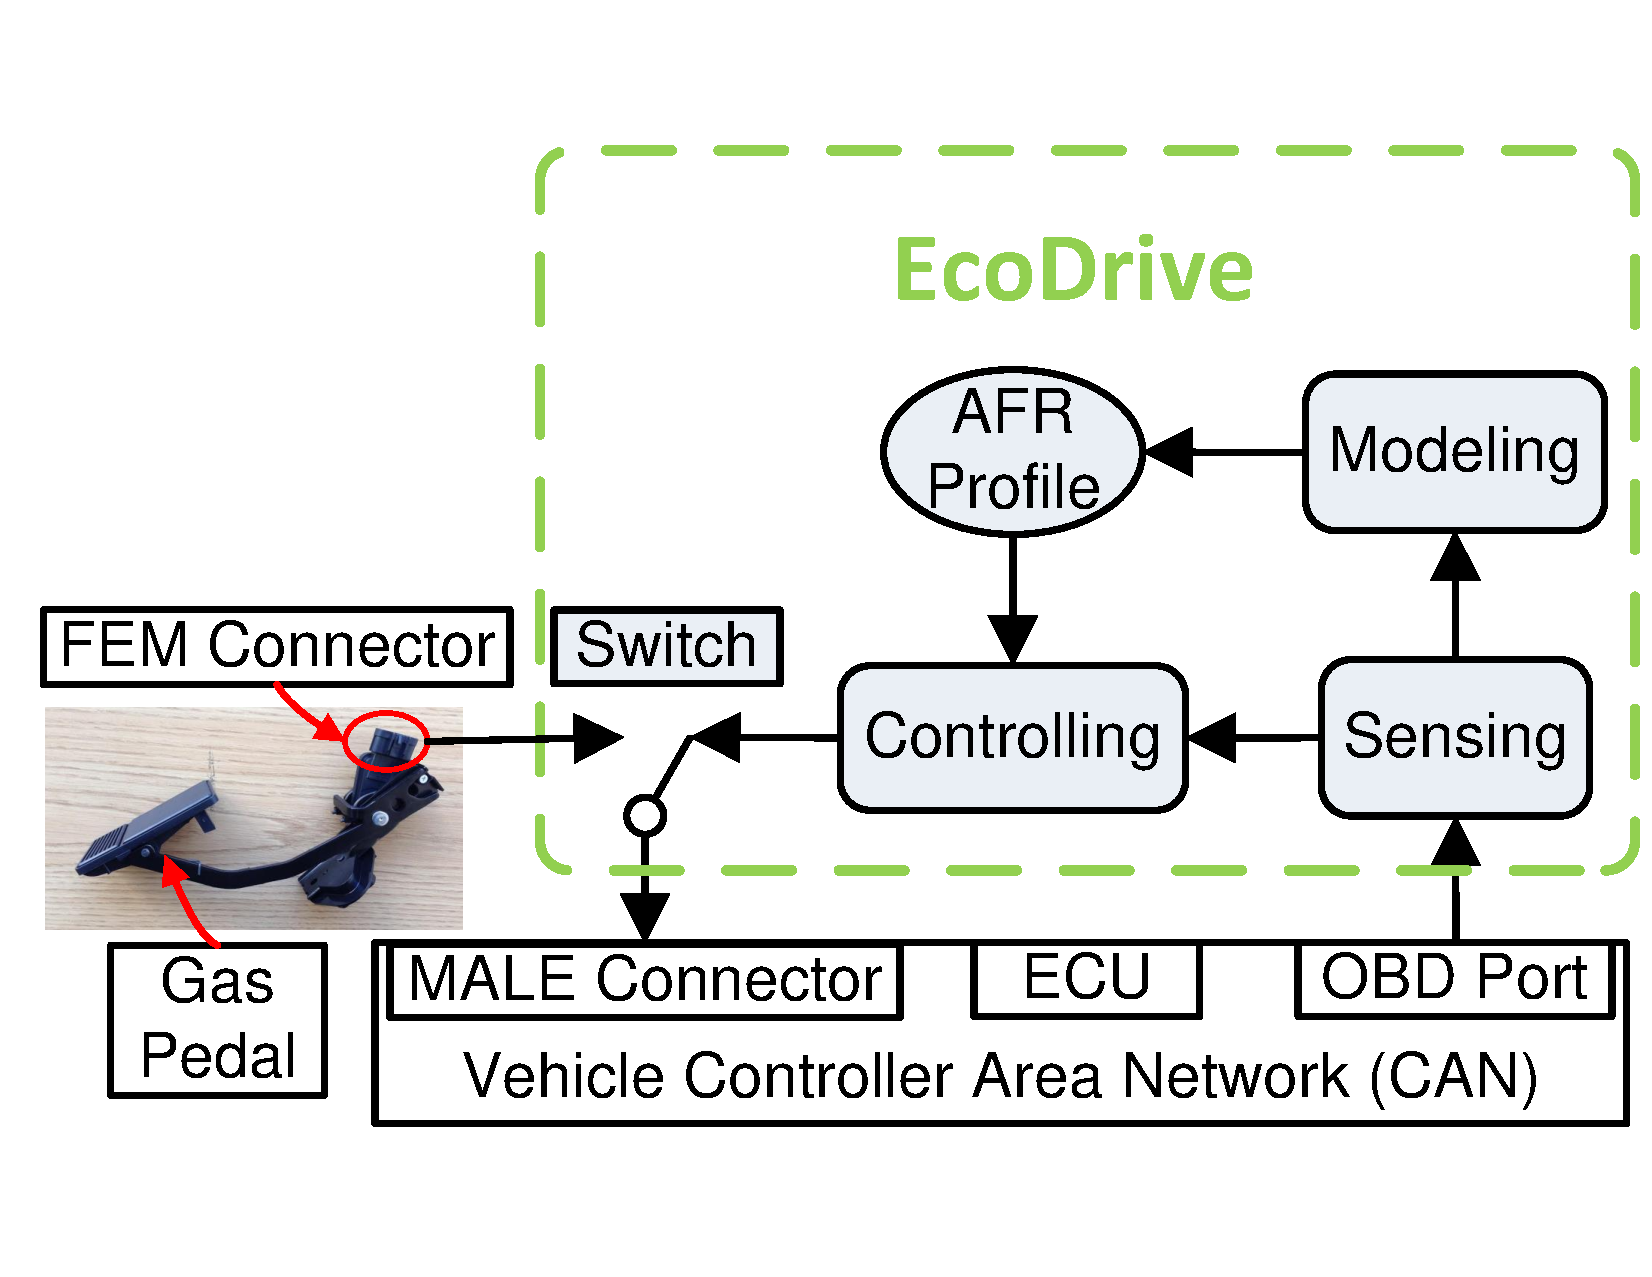
\includegraphics[width=4.0in,angle=0]{Figs/EcoDrive/architecture.pdf}
\vspace{-0.5cm}
\caption{EcoDrive Architecture.}
\vspace{-0.7cm}
\label{ecodrive}
\end{center}
\end{figure}


EcoDrive estimates instant fuel consumptions of different driving behaviors
based on sensed vehicle parameters from the On-board diagnostics (OBD) port \cite{obd, pid}. 
It can adjust vehicular speed in real time according to 
individual vehicle properties and road conditions 
to achieve higher fuel efficiency measured by Kilometer Per Liter (KPL)
\footnote{KPL refers to the distance travelled per unit volume of fuel consumed. 
It interchangeable with Mile Per Gallon (MPG), i.e., 1 KPL = 2.35214583 MPG.}.
EcoDrive is an independent system that can be installed on or removed from 
regular vehicles easily. 
This system controls the vehicle's acceleration and speed 
to provide a fuel efficient drive on its path. 
In our work and current implementation, 
we design this system assuming there is no other factors that 
would contribute to a choice of acceleration and speed, 
e.g., other vehicles, pedestrians, etc. or other obstacles in vicinity. 
Clearly in a practical system, this knowledge would be critical in modifying the acceleration behavior. 
Currently, we adopt the approach followed by other equivalent systems, 
such as cruise control \cite{cruise_control}, which allows the driver to instantly 
disable cruise control by actively pressing the brake pedal. 
In an analogous way, in our current implementation, 
we provide the driver a switch which can be pressed to instantly disable EcoDrive, 
if its acceleration behavior is perceived to be unsafe for nearby vehicles or obstacles.






\textbf{EcoDrive Components}. 
EcoDrive delivers its design via three components including an OBD sensing component, 
a vehicle dynamics modeling component and an acceleration controlling component. 
The architecture is illustrated in Fig. \ref{ecodrive}. 
The sensing component reads real-time OBD parameters through
the OBD port. 
The modeling component models various vehicle forces 
as functions of instant fuel consumption and produces
a fuel consumption profile, called Air/Fuel Rate (AFR) profile
\footnote{AFR refers to the volume of air/fuel cost per unit time.}.
The controlling component utilizes the AFR profile to calculate fuel efficient
driving strategies according to speed limit and road conditions. 
EcoDrive emulates the gas pedal by sending voltage values to 
the connector through an Arduino board.
The vehicular Electronic Control Unit (ECU) controls air/fuel injection rate
according to the voltage inputs. 

EcoDrive addresses two main challenges. 


%\textbf{How to model vehicle dynamics and build AFR profile by using OBD parameters, 
%given various vehicle types, transmission types and road conditions?}
\textbf{a) Model Vehicle Dynamics based on OBD Parameters}.
EcoDrive uses the OBD parameters delivered by
the sensing component to build an AFR profile, 
which records instant fuel consumptions of various accelerations under different speeds. 
To this end, EcoDrive models various vehicle forces, 
including propulsion, drivetrain loss, wind resistance
and grade resistance, as functions of instant fuel consumption.  
First, we model propulsion (or output torque) as a function of engine
torque and gear ratio \cite{vong2006prediction, giannelli2005heavy}. 
We use AFR to model engine torque, and use the ratio between RPM
and vehicular speed to model gear ratio. 
Second, we represent drivetrain loss and wind resistance as a function
of vehicular speed \cite{andersson2012online}.
The coefficients are estimated from recorded data traces where
the car is driving at constant speeds. 
The basic idea is that the sum of resistances is equal to
propulsion when the car is driving at a steady-state speed. 
Third, we model grade resistance by altitude changes over road segments. 
The altitudes of the locations are obtained from 
National Elevation Dataset \cite{nationalelevation}.   
Based on the three models, AFR is modeled as a function of 
speed, acceleration and road conditions. 


\textbf{b) Control Air/Fuel Rate and Vehicular Speed to Improve Fuel Efficiency}.
%\textbf{How to control accelerations and cruising speeds to improve
%gas mileage, given various road segment lengths and speed limits?}
EcoDrive controls vehicular speed by emulating gas pedal. 
It sends the emulated gas pedal position values to the
Arduino board which then converts the position
values to corresponding output voltages.
The output voltages are delivered to the ECU through a 6 Pin Connector.  
The problem is how to adjust vehicular speeds to travel through
a certain distance with the lowest fuel consumption.
We solve this problem by using dynamic programming. 
Each state of the dynamic programming model records 
the minimum air/fuel cost that allows the car to achieve
the current speed at the current location. 
In this model, speed can only increase and the last state of each
speed records the minimum fuel consumption if the car reaches the pre-assigned distance at that speed. 
We call the speed with minimum fuel consumption the target speed.  
By backtracking the state matrix from the last state
of target speed, EcoDrive can obtain the desired AFR at each speed. 
EcoDrive adjusts air/fuel injection rate based on real-time sensed vehicular speed. 
Once the vehicular speed reaches the target speed, EcoDrive
enters a cruising state and commands a constant air/fuel injection rate
until the car reaches the pre-assigned distance. 



\textbf{EcoDrive Prototype}. We build a prototype of EcoDrive in an off-the-shelf mobile embedded platform. 
The prototype is installed and tested on a 2011 Chevrolet Impala. 
We test EcoDrive on the Impala for more than 100 miles in both urban and highway environments.
We evaluate the fuel consumption of EcoDrive and human drivers on different road segments.   
In urban areas, EcoDrive achieves 10\%-40\% higher fuel efficiency than four recruited human drivers.
On highway, we evaluate EcoDrive on two highway segments with different target speeds.    
In our user tests, EcoDrive has over 30\% improvements compared to different human drivers. 
In comparison with cruise control, which is more fuel efficient
than human drivers in the traces we collected, 
EcoDrive achieves an average of 10\% higher fuel efficiency.  
We evaluate the performance of EcoDrive on other vehicles by using trace-driven simulation
based on the 10,000 miles data collected from 12 different vehicles. 
We further find that instant
fuel economy display on regular vehicles is misleading and cruise
control is fuel consuming during speed changes (either requested
by user or affected by road conditions).  






\section{RTDrive: Augmenting Self-Driving with Remote Control}


A self-driving vehicle is one that is capable of sensing 
its environment and navigating itself without human input \cite{wikiselfdrivingcar}. 
It uses a variety of techniques to sense its surroundings,
such as LIDAR, RADAR, odometry, and computer vision. 
It uses these different sensor inputs 
to understand its environment, 
recognize various road conditions, traffic lights, road signs,
lane boundaries, and track surrounding vehicles.
The potential benefits of self-driving vehicles
include increased safety, increased mobility and lower
costs. 
It is estimated that self-driving vehicles can reduce 90\%
of the accidents and prevent up to \$190 
billion in damages and health-costs annually
\cite{litman2014autonomous}.


Many commercial and academic endeavors are putting significant resources
for the development and tests
of such self-driving systems \cite{waymo, benz, autox}.
For example, Google started its self-driving project in 2009,  
and has spent more than \$1 billion
in building and testing fully self-driving vehicles~\cite{googlespend}. 
While legal and political challenges remain in its widespread adoption,
there are also some technical bottlenecks on the way of developing
completely reliable self-driving systems.


All self-driving systems make
decisions based on the perception of the environment and
predefined traffic rules. However, there has been occasional
failures of these systems when they have encountered scenarios
that were hitherto unseen. For instance, based on the situation
 in a construction
zone, human drivers would realize that it is permissible to cross
over a double yellow line by following the appropriately placed
cones  (which otherwise is illegal to cross
in the US), while a self-driving vehicle may not be able to
do so, and therefore be unable to move forward. Similarly in
poor weather conditions or due to traffic light malfunctions,  
the cues from different sensors may
contradict each other leading to confusion in decision making.

In general, the road rules are complex and may conflict with
each other, i.e., the system has to understand when
to follow cones and ignore lane markers, 
and when to obey a road worker and disobey traffic
signs.
%To address the last mile challenge, some recent work \cite{kang2018rc} 
%propose to use specially designated remote human operators
%to augment self-driving system when it fails to 
%perceive or handle current situations. 
While it is tempting to return control (during the failure of the self-driving
function) to a local human driver situated in the vehicle, 
it is foreseeable a future of driverless cabs carrying only
underage or licenseless passengers.
Hence, we expect that remote drivers can multiplex and manage
a large group of vehicles making scalability feasible.
However, accomplishing remote driving for a vehicle requires careful tuning 
of (wireless-based) network parameters, media content and their formats,
and control experience with some real-time constraints between the vehicle 
and the remote driving station.

%It is well established that human
%drivers, especially experts, are capable of making good judgement calls
%in face of contradictory or inadequate inputs, that sometimes limit 
%a learning system that has yet to encounter a scenario before.
%While it is tempting to return control (during the failure of the self-driving
%function) to a local human driver situated in the vehicle, 
%it is foreseeable a future of driverless cabs carrying only
%underage or licenseless passengers.
%Hence, we expect that remote drivers can multiplex and manage
%a large group of vehicles making scalability feasible.



In this paper, we present RTDrive, a remote driving framework
that augments self-driving system when it fails to 
percept and/or handle current situations. 
RTDrive consists of a live streaming system
and a remote control server. 
The live streaming system can encode videos by using
a context-aware video encoding algorithm. 
It also includes a live streaming protocol that 
carries out a consistent-latency
view mechanism to make the view of the operator
more smooth. 
The framework also consists of several modules, video codec, 
Forward Error Correction (FEC), vehicle dynamics sensing,
lane boundary detection, object detection etc.,
that enable further extension, optimization and innovation.  



\textbf{Context-Aware Video Encoding}.
The context-aware video encoding algorithm can 
sense vehicle dynamics and based on which it 
selects the optimal video encoding bitrate and key frame intervals. 
In video live streaming, the video is encoded into two
frames, I-frame and P-frame.
I-frame is also called key frame and it can be 
decoded into a complete image. 
P-frame only encodes the difference between current
frame to previous I-frames and P-frames. 
The context-aware video encoding algorithm
can dynamically adjust the number of I-frames
and P-frames to improve video encoding efficiency. 
The intuition is to adjust the key frame interval 
based on the frequency of camera view changes. 
For example, in the cases of turning or high speed scenarios,
there should be more I-frames since P-frames cannot
carry enough information which may lead to severe quality degradation. 
Through real world trip data collection and replay,
the context-aware video encoding algorithm can outperform
the default encoding algorithm by 10\%-30\% in various trips. 

\textbf{Live Streaming Protocol}.
We design and implement a live streaming protocol. 
It consists of several modules such as UDP/TCP, FEC, 
bandwidth and packet loss rate estimation. 
We discuss the design choices and evaluate these modules
under various network parameter settings. 
Also, a consistent-latency view algorithm 
is designed to deliver smooth
videos to improve the remote control experience. 
It uses a buffer to order the frames based on the timestamps
and deliver to the frame display engine only when it is 
the its order.
It achieves this goal by tracking two parameters, 
the latency difference and the latency deviation.   
The latency difference between
the live streaming system and the server is
tracked by using a low pass filter. 
The deviation of the latency difference is also recorded. 
Through a user study with 20 participates on controlling the Android-powered
vehicle, the operators with consistent-latency have
2x better control precision. 


This paper makes the following contributions:
\begin{itemize}
\setlength\itemsep{0em}

\item We design and implement RTDrive, a live streaming and remote control
framework, that can be used to view video stream and
control the vehicle remotely in real time. 
RTDrive can augment self-driving systems when they are
failed to percept the environment under various unpredictable conditions. 

\item We present a context-aware video encoding algorithm,
which can encode video frames according to vehicle dynamics. 
According to the traces we collected, it is able to improve
the video encoding efficiency by 10\% to 30\% on average in 
various driving scenarios. 

\item We propose a consistent-latency live streaming protocol,
which can adapt to wireless network conditions and buffer frames
for smooth display. 
It includes various modules such as bandwidth estimation, loss rate 
estimation, FEC encoding and frame buffering. 
According to a user study with 20 participates, 
the consistent-latency view algorithm improve the control
precision by more than 2x on average in a parking
task. 
\end{itemize}





\section{Contributions}


This thesis work makes the following contributions:
\begin{itemize}
\setlength\itemsep{0em}


\item We illustrate that the accuracy of smartphone built-in sensors are very sensitive
to road conditions and human interactions when conducting driving analytics. 
Traditional slope-unaware approach may caused misalignment and acceleration over/under
estimation, which may cause significant sensing errors. 
We develop several techniques to identify the usability and accuracy of inertial sensors 
and improve their performance.  
We consider using commodity mobile device GPS receivers to sense vehicle
motion parameters, especially those related to acceleration and brakes, 
and evaluate the performance by more than 
10,000 miles of driving data. 
We find that GPS can be a good candidate to estimate such vehicle
motions, especially in high speed scenarios (higher than $10m/s$ or $22mph$). 
It indicates that GPS can be a good alternative than inertial
sensors due to its simplicity and better performance in high speed
scenarios.  
We develop DriveSense, an Android application component that can 
selectively use GPS and inertial sensors for driving analytics. 
A beta version of DriveSense has been released to 9 volunteers and this version has
currently recorded more than 3,000 miles of driving data in the last six months.
Our evaluation shows that DriveSense can improve the overall performance 
comparing with using either GPS or well-tuned inertial sensors. 



\item We design and implement EcoDrive, 
which is an independent fuel consumption sensing and control system
that can improve fuel efficiency. 
The system is implemented on an embedded platform 
that can be easily installed on regular vehicles. 
We model various vehicle forces as functions of instant fuel consumption
and the models are evaluated by utilizing 
10,000 miles of driving traces collected from 12 vehicles. 
EcoDrive is installed on a regular vehicle and evaluated by more than 100 miles of driving in both urban and highway environments, 
and demonstrated to improve fuel efficiency compared to cruise control system
of the vehicle and to human drivers.  




\item We design and implement RTDrive, a live streaming and remote control
framework, that can be used to view video stream and
control the vehicle remotely in real time. 
RTDrive can augment self-driving systems when they are
failed to percept the environment under various unpredictable conditions. 
It includes a context-aware video encoding algorithm,
which can encode video frames according to vehicle dynamics. 
According to the traces we collected, it is able to improve
the video encoding efficiency by 10\% to 30\% on average in 
various driving scenarios. 
It also includes a consistent-latency live streaming protocol,
which can adapt to wireless network conditions and buffer frames
for smooth display. 
It includes various modules such as bandwidth estimation, loss rate 
estimation, FEC encoding and frame buffering. 
According to a user study with 20 participates, 
the consistent-latency view algorithm improve the control
precision by more than 2x on average in a parking
task. 




\end{itemize}






\section{Outline}

The rest of the thesis is organized as follows. 
In Chapter \ref{chapter_drivesense}, we present
our driving analytics system DriveSense, which leverages smartphone
sensors to monitor driving behaviors.
In Chapter \ref{chapter_ecodrive}, we present EcoDrive, an in-vehicle
system that can . 
In Chapter \ref{chapter_rtdrive}, we propose the live streaming
and remote control framework RTDrive, which can augment
self-driving systems upon occational failures. 
In Chapter \ref{chapter_relatedwork}, we compare our work with prior
approaches and systems to monitor, assist or even replace human
drivers. 
We conclude and discuss the avenues for further research in Chapter \ref{chapter_conclusion}.



